\documentclass[final,ngerman,ignorenonframetext,compress]{beamer}
% \includeonlyframes{current}
\usepackage{garamond}
\usepackage{listings}
\usepackage{booktabs}
\usepackage{ulem}

\lstset{language=python,keywordstyle=\color{beamer@bonnblue},emphstyle=\color{red},showstringspaces=false}

\mode<beamer>
{%
  \usetheme{Bonn}
  \pgfdeclareimage[height=0.8cm]{university-logo}{Logo_UBo_h24_4c-crop}
  %\setbeamertemplate{footline}[default]
  \logo{\pgfuseimage{university-logo}}
  \setbeamertemplate{navigation symbols}{}
}
\mode<handout>{%
  \usetheme{default}
  \usecolortheme{dove}
  \setbeamercolor{background canvas}{bg=black!5}
  \usepackage{pgfpages}
  \pgfpagesuselayout{8 on 1}[a4paper,border shrink=5mm]
}

%\setbeamerfont{title}{family*=ugm}
%\setbeamerfont{frametitle}{family*=ugm}

\DeclareMathOperator*{\mymax}{max}
\DeclareMathOperator*{\argmax}{arg\,max}
\DeclareMathOperator*{\argmin}{arg\,min}
\DeclareMathOperator{\cov}{cov}
\DeclareMathOperator{\sign}{sign}
\DeclareMathOperator{\dist}{dist}
\DeclareMathOperator{\freq}{frequency}
\DeclareMathOperator{\selcrit}{selcrit}
\DeclareMathOperator{\precision}{precision}
\DeclareMathOperator{\recall}{recall}
\DeclareMathOperator{\neighbours}{neighbours}
\DeclareMathOperator{\desclen}{descriptionlength}

\newcommand\itplus{\kreis{$+$}{green}}
\newcommand\itminus{\kreis{$-$}{red}}
\newcommand\w[1]{\ensuremath{\mathbf{#1}}}

% avant, courier, chancery, times, palatino, bookman
% newcent, utopia, charter
\usepackage[ngerman]{babel}
\usepackage{times}

\usepackage[latin1]{inputenc}
\usepackage[T1]{fontenc}
% \usepackage{psfrag}
\usepackage{multicol}
\usepackage{mdwtab}
\usepackage{txfonts,textcomp}
\usepackage{amsmath}
\usepackage{amsfonts}

\setlength\parindent{0cm}
\setlength\parskip{2mm}
\setbeamerfont{gross}{size=\large}
\setbeamerfont{quetsch}{size=\tiny}
\setbeamerfont{klein}{size=\footnotesize}

% example list spacing
\newcommand\ml{\setlength\itemindent{-11mm}}

%\titlegraphic{\includegraphics[width=2cm,height=2cm]{Blackheaded_python2}}

% \DeclareGraphicsRule{.jpg}{eps}{.bb}{`bmeps -c #1}

\title[Wurzelstrukturerkennung]{Wurzelstrukturerkennung aus NMR-Daten}

\author[Schulz, Behnke]{Hannes Schulz, Sven Behnke}
\institute[Uni Bonn, Germany]%
{
\includegraphics[width=.2\linewidth]{Logo_UBo_h24_4c-crop}}
%{Rheinische Friedrich-Wilhelms-Universität Bonn}

\date{28. Februar 2011}


%\beamerdefaultoverlayspecification{<+->}

\begin{document}

\begin{frame}[plain]
	\titlepage%
\end{frame}


\begin{frame}[plain] % WipeBlobs
	\frametitle{Outline}
		\begin{columns}
			\column{.8\linewidth}
			\tableofcontents[hidesubsections]
		\end{columns}
	% You might wish to add the option [pausesections]
\end{frame}

\section{Beschreibung der Daten}

\begin{frame}
	\frametitle{Untersuchungsobjekt}
	\begin{columns}
		\column{.5\linewidth}
		\begin{center}
			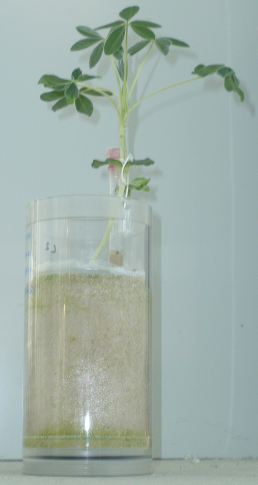
\includegraphics[width=.6\linewidth]{img/o2}
		\end{center}
		\column{.5\linewidth}
		\begin{itemize}
			\item Lupine
			\item Natursandboden
		\end{itemize}
	\end{columns}
\end{frame}

\begin{frame}
	\frametitle{NMR-Daten von Andreas Pohlmeier}
	\begin{columns}
		\column{.4\linewidth}
		\begin{itemize}
			\item Multi-Slice Aufnahme ($256\times256\times120$)
			\item Verschiedene Stadien (Wachstum, Stress)
		\end{itemize}
		\vspace{1cm}

		\begin{center}
			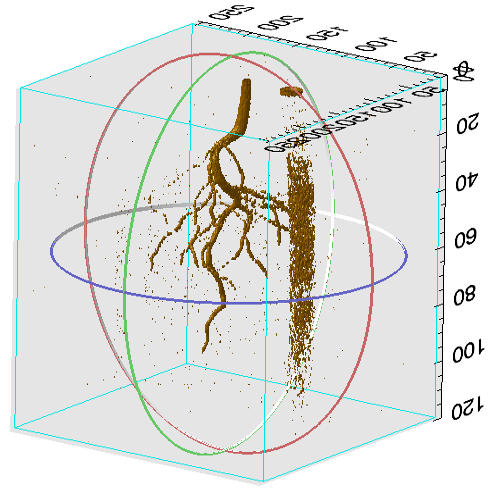
\includegraphics[width=.7\linewidth]{img/d1}
		\end{center}
		\column{.4\linewidth}
		\begin{center}
			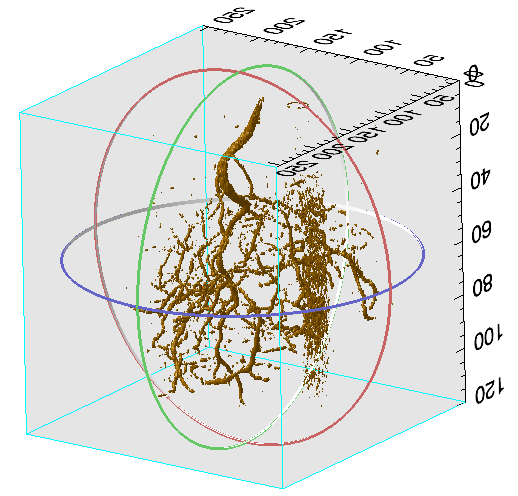
\includegraphics[width=.7\linewidth]{img/d2}\\
			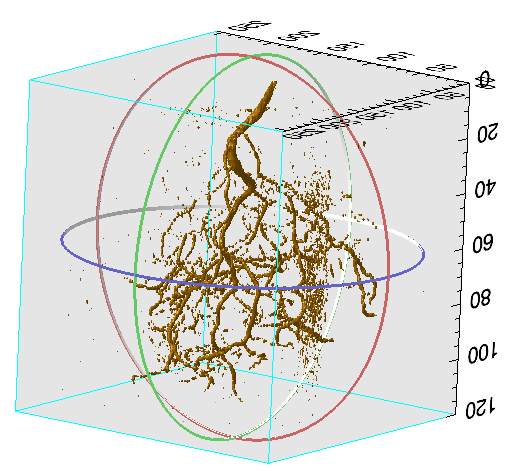
\includegraphics[width=.7\linewidth]{img/d3}
		\end{center}
	\end{columns}
\end{frame}

\begin{frame}
	\frametitle{NMR-Daten}
	\begin{columns}
		\column{.5\linewidth}
		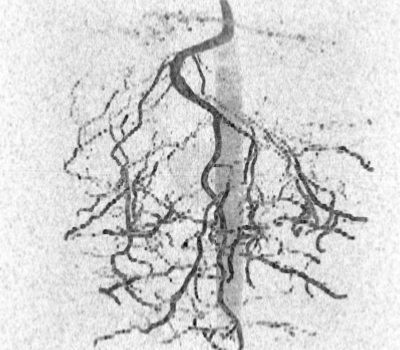
\includegraphics[width=\linewidth]{img/raw-4.png}
		\column{.5\linewidth}
		\begin{itemize}
			\item Pixelhelligkeit $\propto$ Wassergehalt
			\item Wurzel $\approx$ 80\%
			\item Boden $\approx$ 10\%  (Natursand)
			\item Verunreinigungen (Eisen) st\"oren Signal
			\item Wassergef\"ulltes Messr\"ohrchen aus Glas
			\item Aufnahmedauer 1-3h
		\end{itemize}
	\end{columns}
\end{frame}

\section{Aufgabenstellungen}

\begin{frame}
	\frametitle{Aufgabenstellungen}
	\begin{columns}
		\column{.5\linewidth}
		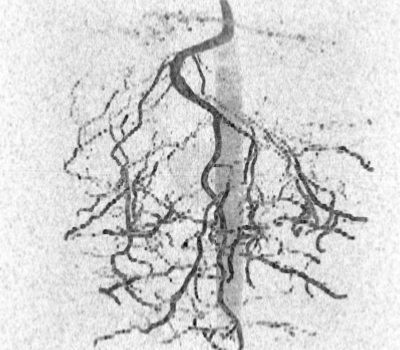
\includegraphics[width=\linewidth]{img/raw-4.png}
		\column{.5\linewidth}
		\begin{itemize}
			\item Wassergehalt in der Wurzel modellieren
			\item Wachstum beschreiben
			\item Wurzel-L\"angen-Dichte bestimmen
			\item<alert@2> Zur Zeit: Manuelle Annotation in VR-Toolkit ($\approx$7h)
		\end{itemize}
	\end{columns}
\end{frame}

\section{L\"osungsansatz zur Bestimmung der Wurzelkonnektivit\"at}
\begin{frame}
	\frametitle{1. Entfernen des R\"ohrchens}
	\begin{columns}
		\column{.5\linewidth}
		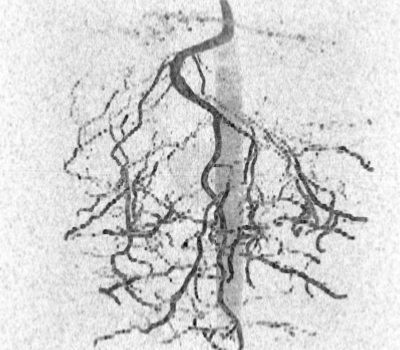
\includegraphics[width=\linewidth]{img/raw-4.png}
		\column{.5\linewidth}
		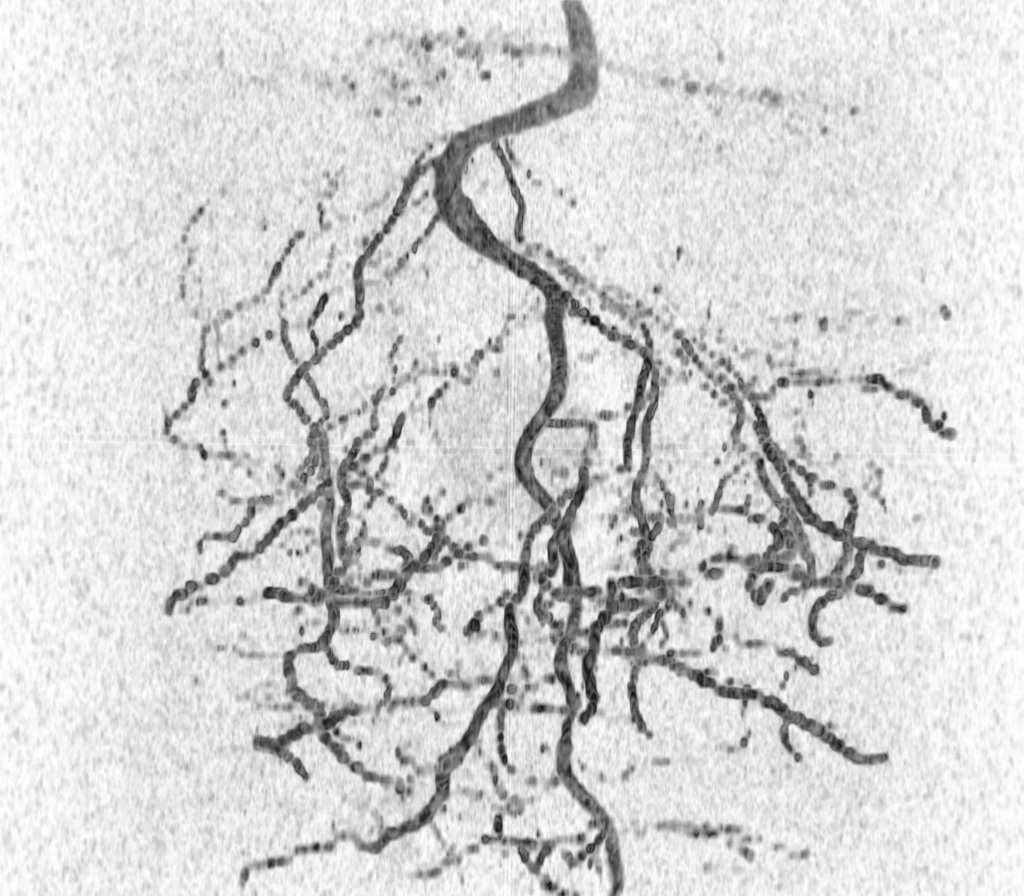
\includegraphics[width=\linewidth]{img2/raw-4.png}
	\end{columns}
\end{frame}

\begin{frame}
	\frametitle{2. Finden von r\"ohren\"ahnlichen Strukturen}
	\begin{columns}
		\column{.5\linewidth}
		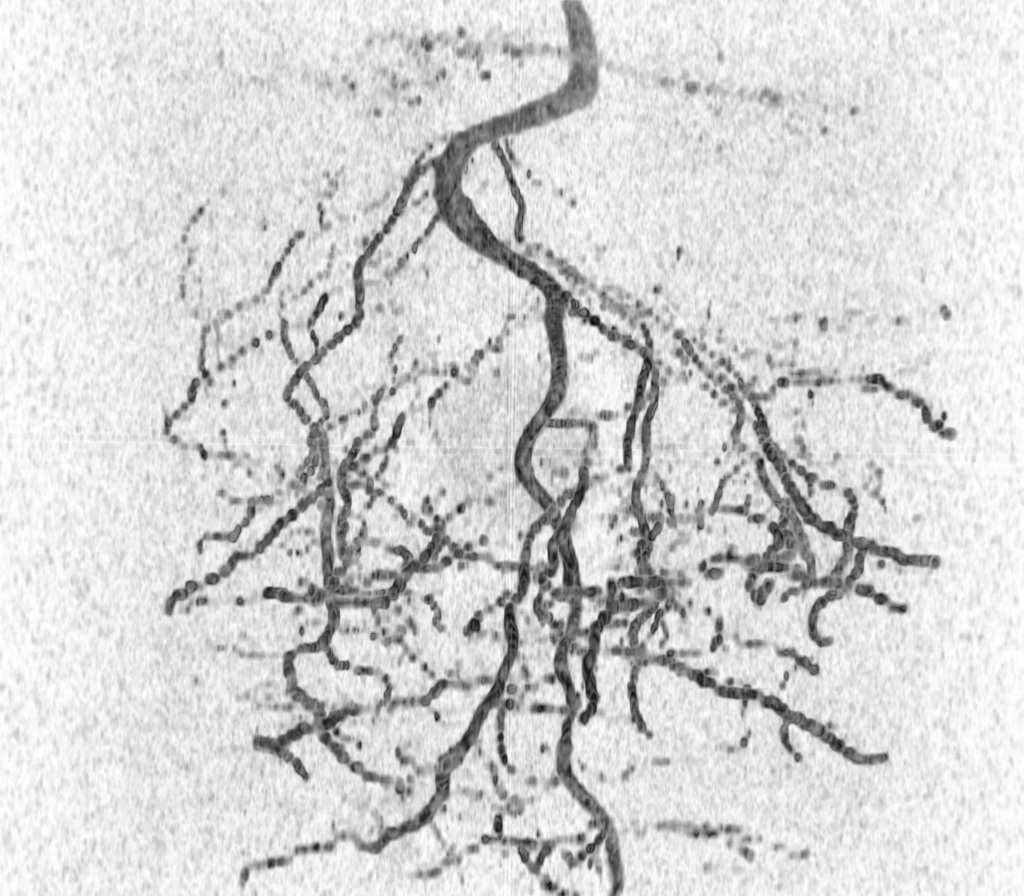
\includegraphics[width=\linewidth]{img2/raw-4.png}
		\column{.5\linewidth}
		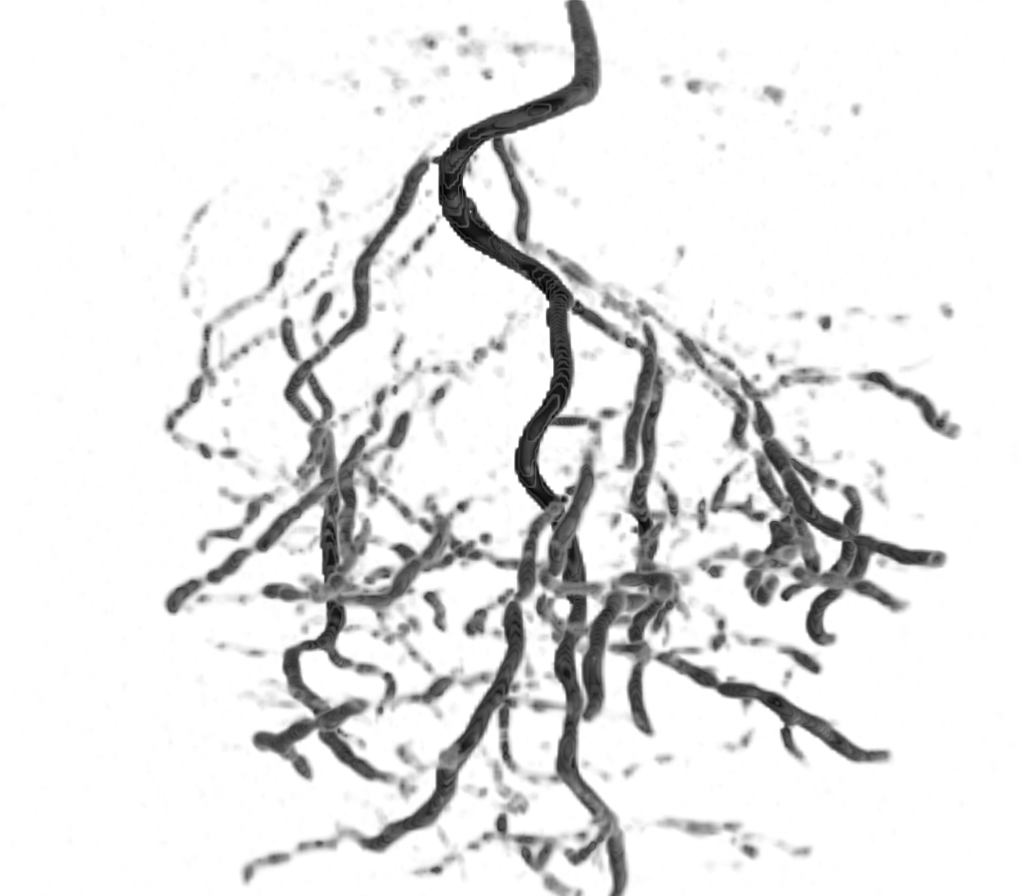
\includegraphics[width=\linewidth]{img2/sato-bone-4.png}
	\end{columns}
	\begin{center}	
		Multi-Scale Verfahren basierend auf Eigenwerten der lokalen Hesse-Matrizen.
		Details in Sato et al. 1997, Frangi et al. 1998
	\end{center}
\end{frame}

\begin{frame}
	\frametitle{3. Verfolgen der gefundenen R\"ohren}
	\begin{columns}
		\column{.5\linewidth}
		\begin{itemize}
			\item Manuelles Bestimmen eines Punktes $P$ in der
				Hauptwurzel
			\item Definiere Graph auf Voxelgrid
				Kantengewicht $w_{ij}=\exp(-\alpha s_j)$
			\item Finde k\"urzeste Distanz f\"ur jeden Voxel zu $P$
			\item Auswahl von Startpunkten basierend auf
				Rohdaten und durchschnittlichem Kantengewicht
		\end{itemize}
		\column{.5\linewidth}
		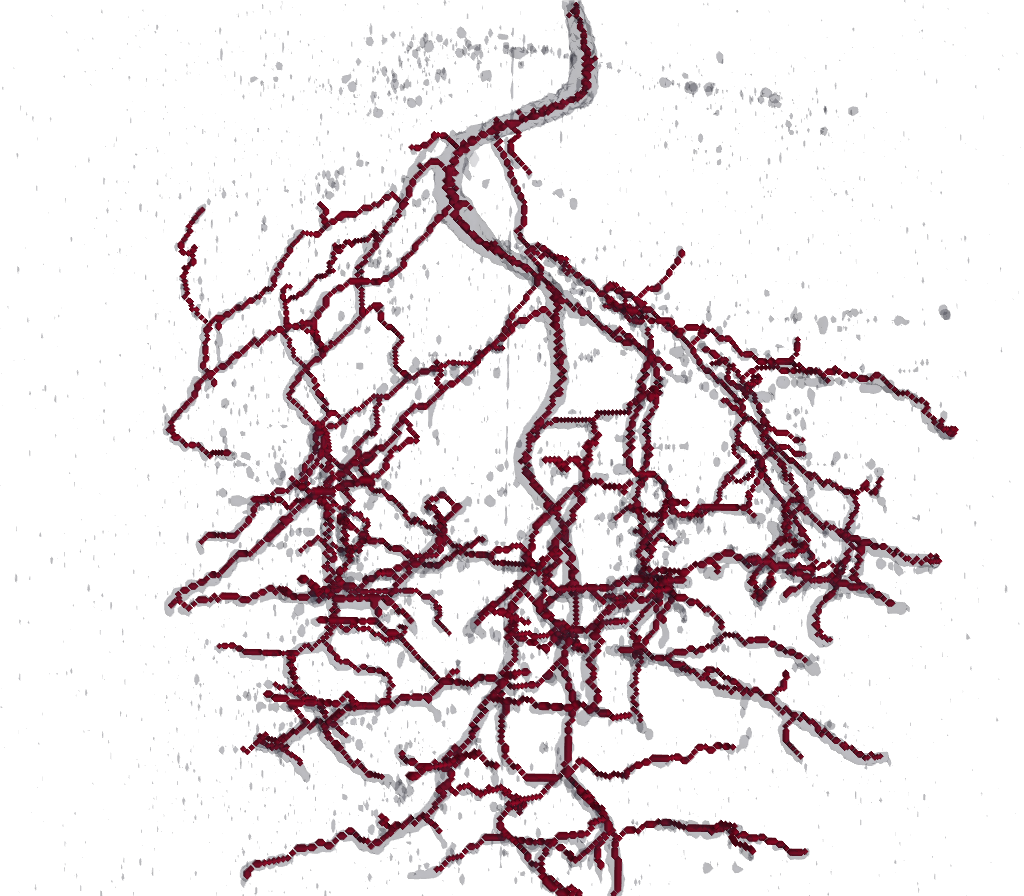
\includegraphics[width=\linewidth]{img2/rendered-paths-4.png}

		\begin{center}
			Gerenderte Pfade
		\end{center}
	\end{columns}
\end{frame}

\begin{frame}
	\frametitle{4. Skelettieren der Pfade}
	\begin{columns}
		\column{.5\linewidth}
		\begin{itemize}
			\item Behalte nur Knoten $n$ mit
				\begin{itemize}
					\item R\"ohrchen\"ahnlichkeitsbild($n$) ist lokales Maximum
					\item Out-Degree$(n)>1$
				\end{itemize}
		\end{itemize}
		\column{.5\linewidth}
		\includegraphics<1>[width=\linewidth]{img2/path-ours-4.png}
	\end{columns}
\end{frame}

\begin{frame}
	\frametitle{Vergleich mit von-Hand gelabelter Wurzel}
	\begin{columns}
		\column{.5\linewidth}
		\includegraphics<1>[width=\linewidth]{img2/path-traces-4.png}
		\column{.5\linewidth}
		\includegraphics<1>[width=\linewidth]{img2/raw-4.png}
	\end{columns}
\end{frame}

\begin{frame}[plain]
	\begin{center}
		\Huge{Fragen?}
	\end{center}
\end{frame}

\end{document}

% vim:autoread
